\documentclass{beamer}
\usepackage{lmodern}
\usetheme{Copenhagen}
\setbeamertemplate{headline}{}
\newcounter{saveenumi}
\newcommand{\seti}{\setcounter{saveenumi}{\value{enumi}}}
\newcommand{\conti}{\setcounter{enumi}{\value{saveenumi}}}
\usepackage[]{graphicx}\usepackage[]{xcolor}
% maxwidth is the original width if it is less than linewidth
% otherwise use linewidth (to make sure the graphics do not exceed the margin)
\makeatletter
\def\maxwidth{ %
	\ifdim\Gin@nat@width>\linewidth
	\linewidth
	\else
	\Gin@nat@width
	\fi
}
\makeatother

\definecolor{fgcolor}{rgb}{0.345, 0.345, 0.345}
\newcommand{\hlnum}[1]{\textcolor[rgb]{0.686,0.059,0.569}{#1}}%
\newcommand{\hlstr}[1]{\textcolor[rgb]{0.192,0.494,0.8}{#1}}%
\newcommand{\hlcom}[1]{\textcolor[rgb]{0.678,0.584,0.686}{\textit{#1}}}%
\newcommand{\hlopt}[1]{\textcolor[rgb]{0,0,0}{#1}}%
\newcommand{\hlstd}[1]{\textcolor[rgb]{0.345,0.345,0.345}{#1}}%
\newcommand{\hlkwa}[1]{\textcolor[rgb]{0.161,0.373,0.58}{\textbf{#1}}}%
\newcommand{\hlkwb}[1]{\textcolor[rgb]{0.69,0.353,0.396}{#1}}%
\newcommand{\hlkwc}[1]{\textcolor[rgb]{0.333,0.667,0.333}{#1}}%
\newcommand{\hlkwd}[1]{\textcolor[rgb]{0.737,0.353,0.396}{\textbf{#1}}}%
\let\hlipl\hlkwb

\usepackage{framed}
\makeatletter
\newenvironment{kframe}{%
	\def\at@end@of@kframe{}%
	\ifinner\ifhmode%
	\def\at@end@of@kframe{\end{minipage}}%
\begin{minipage}{\columnwidth}%
	\fi\fi%
	\def\FrameCommand##1{\hskip\@totalleftmargin \hskip-\fboxsep
		\colorbox{shadecolor}{##1}\hskip-\fboxsep
		% There is no \\@totalrightmargin, so:
		\hskip-\linewidth \hskip-\@totalleftmargin \hskip\columnwidth}%
	\MakeFramed {\advance\hsize-\width
		\@totalleftmargin\z@ \linewidth\hsize
		\@setminipage}}%
{\par\unskip\endMakeFramed%
	\at@end@of@kframe}
\makeatother

\definecolor{shadecolor}{rgb}{.97, .97, .97}
\definecolor{messagecolor}{rgb}{0, 0, 0}
\definecolor{warningcolor}{rgb}{1, 0, 1}
\definecolor{errorcolor}{rgb}{1, 0, 0}
\newenvironment{knitrout}{}{} % an empty environment to be redefined in TeX

\usepackage{alltt}
%\usepackage{fullpage}
\usepackage{graphicx}
\usepackage[utf8]{inputenc}
\usepackage{amsmath}
\usepackage{graphics}
\usepackage{float}
\usepackage{xcolor}
\usepackage{geometry}
\usepackage{tikz}
\usetikzlibrary{shapes, arrows}
\usepackage[utf8]{inputenc}
\usepackage{amsmath}
\usepackage{graphics}
\usepackage{xcolor}
\usepackage{hyperref}
\usepackage{longtable}
\usepackage{array}
\usepackage{adjustbox}
\numberwithin{equation}{section}
\numberwithin{table}{section}
\IfFileExists{upquote.sty}{\usepackage{upquote}}{}
\title{Modeling Depression Severity among Caregivers in a Rural Setting using Multiple Linear Regression}

\author[]{BEVERLY KIND : \hspace{0.2cm}    I63/4240/2019 \\ CHARLES WAMBUA : \hspace{0.2cm}     I63/4248/2019\\ ODHIAMBO KENNEDY : \hspace{0.2cm}    I63/4282/2019\\ PERTER DOKTA : \hspace{0.2cm}    I63/136668/2019\\DOMINIC NYAENYA : \hspace{0.2cm}    I63/4261/2019\\ \vspace{0.2cm} \textbf{SUPERVISOR}: DR. MUSIGA}
\institute[]{
\includegraphics[width=0.1\textwidth]{UoN_Logo.png}}
\date{June 16, 2023}
\begin{document}
\maketitle
\section{INTRODUCTION}
\begin{frame}{Background Information}
\begin{itemize}
\item Depression is a mental health disorder characterized by persistent feelings of sadness, loss of interest or pleasure in activities, changes in appetite or sleep patterns, fatigue, difficulty concentrating, and thoughts of self-harm or suicide.

\item   It is a complex condition that can significantly impact individuals' emotional well-being, cognitive functioning, and overall quality of life. 

\item  Depressed individuals may have difficulty concentrating and making decisions, which can hinder their productivity in various aspects of life. 

\item  Rehabilitation centers for depression have been established to provide specialized treatment facilities that provide comprehensive care for individuals experiencing moderate to severe depression
\end{itemize}
\end{frame}
\begin{frame}{Statement of the Problem}
Researchers have been faced with the problem of identifying potential predictors of depression among cancer caregivers.
The problem is to identify and to quantify the important variables linked to depression.
\end{frame}
\begin{frame}{Objective of the Study}
\begin{block}{General objectives}
	\vspace{0.4cm}
To model depression severity among caregivers in a rural setting using multiple linear regression model. 
\end{block}
\begin{block}{Specific objectives}
	\begin{itemize}
\item To identify the significant predictors that contribute to depression among cancer caregivers in a rural setting

\item To assess the performance of the multiple linear regression model in predicting depression among cancer caregivers. This involves evaluating the goodness of fit measures.

\item To provide evidence-based recommendations for interventions and support systems aimed at addressing depression among cancer caregivers
	\end{itemize}
\end{block}
\end{frame}

\begin{frame}{Justification of the Study}
	\begin{itemize}
\item  The results of this study can help with the creation and enhancement of rural cancer caregiver support systems.
\vspace{0.6cm}
\item Healthcare professionals, policymakers, and support groups can create targeted treatments that meet the unique needs and difficulties of caregivers in these circumstances by recognizing the predictors of depression.
	\end{itemize}
\end{frame}
\section{LITERATURE REVIEW}
\begin{frame}{Literature Review}
\begin{enumerate}
	\item Jain et al. (2013);
	\begin{itemize}
	\item  Examined the burden of depression on work productivity in the US workforce among 1051 full-time employees in February 2010.
	\item All levels of depression were associated with decreased work productivity as severity increased, presenteeism and absenteeism worsened.
	\end{itemize}

\item Serpa et al. (2014);

\begin{itemize}
\item Investigated the major problems among Veterans specifically anxiety, depression and suicidal ideation among 79 veterans at an urban Veterans Health Administration medical facility. 
\item The results indicated significant reductions in anxiety, depressions, and  suicidal ideation after MBSR training as well as improved mental health functioning scores although pain intensity and physical health functionality did not register improvements
\end{itemize}
\seti
	\end{enumerate}
\end{frame}
\begin{frame}
\begin{enumerate}
	\conti
	\item Laing and Jones (2016)
\begin{itemize}
\item  Investigated the mediation effect of anxiety and depression on the relationship between perceived health-promoting workplace culture and presenteeism among 4703 state employees.
\item  Correlational analysis indicated that indirect effects of workplace culture on productivity, mediated by anxiety and depression symptoms were significant. Healthy living culture and anxiety were significantly negatively associated and anxiety and presenteeism were significantly positively associated.
\end{itemize}
\item Magtibay et al. (2017)
\begin{itemize}
	\item assessed the efficacy of blended learning which was intended to decrease stress and burnout among nurses through the use of the SMART program.
	\item  The results indicated statistically significant, clinically meaningful decreases in anxiety, stress, and burnout and increases in resilience, happiness, and mindfulness.
\end{itemize}
\seti
\end{enumerate}
\end{frame}
\begin{frame}
	\begin{enumerate}
		\conti
		\item Levis et al. (2019)
		\begin{itemize}
			\item Evaluated the accuracy of the Patient Health Questionnaire-9 (PHQ-9) for screening major depression in adults using individual participant data meta-analysis.
			\item The study found that combined sensitivity and specificity was maximized at a cut-off score of 10 or above among studies using a semi-structured interview. Secondly across cut-off scores of 5-15, sensitivity with semi-structured interviews was 5\%-22\% higher than for fully structured interviews.
		\end{itemize}
	\item Leung et al. (2020)
	\begin{itemize}
		\item Investigated the factor structure, reliability, and construct validity of the Patient Health Questionnaire-9 (PHQ-9) in a community sample of 10,933 Chinese adolescents.
		\item The results indicated that a one-factor model with three pairs of items correlations fitted the PHQ-9 data well and that measurement invariances by age and gender were supported. The PHQ-9 was also strongly correlated with anxiety, self-esteem and perceived control.
	\end{itemize}
	\seti
	\end{enumerate}
\end{frame}
\begin{frame}
	\begin{enumerate}
		\conti
		\item Lister et al. (2023)
		\begin{itemize}
			\item conducted a qualitative study that investigated the barriers and enablers to mental wellbeing and academic success that students experienced in distance learning.
			\item The study found that barriers and enablers were existent in the majority of themes, implying that different aspects of study could be both barriers or enablers for mental wellbeing and study success, depending on who was experiencing them and how
		\end{itemize}
	\end{enumerate}
\end{frame}
\section{METHODOLOGY}
\begin{frame}{Multiple Linear Regression Model}
	\begin{itemize}
		\item  Suppose we want to use $k$ predictor variables $X_1, X_2, \ldots, X_k$ to explain a response variable $y$\\
\item   then the model is of the form:
	\end{itemize}
\begin{equation}
	y=\beta_0+\beta_1 X_1+\ldots+\beta_k X_k+\epsilon
	\label{eq:methodology_eq1}
\end{equation}
\end{frame}
\begin{frame}
In matrix form we have
$$
\left[\begin{array}{c}
	y_1 \\
	y_2 \\
	\vdots \\
	y_n
\end{array}\right]=\left[\begin{array}{ccccc}
	1 & x_{11} & x_{12} & \cdots & x_{1 k} \\
	1 & x_{21} & x_{22} & \cdots & x_{2 k} \\
	\vdots & & & & \vdots \\
	1 & x_{n 1} & X_{n 2} & \cdots & x_{n k}
\end{array}\right]\left[\begin{array}{c}
	\beta_0 \\
	\beta_1 \\
	\vdots \\
	\beta_k
\end{array}\right]+\left[\begin{array}{c}
	\epsilon_1 \\
	\epsilon_2 \\
	\vdots \\
	\epsilon_n
\end{array}\right]
$$
i.e
\begin{equation}
	\underbrace{\mathbf{y}}_{n \times 1}=\underbrace{\mathbf{X}}_{n \times(k+1)} \underbrace{\underline{\boldsymbol{\beta}}}_{(k+1) \times 1}+\underbrace{\boldsymbol{\varepsilon}}_{n \times 1}
\end{equation}
\end{frame}
\begin{frame}
where;\\
\begin{itemize}
	\item The matrix $\mathbf{X}$ is called design matrix ;\\

\vspace{0.3cm}
\item  $\underline{\boldsymbol{\beta}}$ is a column vector of regression coefficients.\\
\vspace{0.3cm}
\item  $\mathbf{y}$ is a column of response values for individuals in the sample.\\

\vspace{0.3cm}
\item $\epsilon_i$ is the error term of individual observations of the outcome $y_i$ 
\end{itemize}
\end{frame}

\begin{frame}
\begin{block}{Assumptions of the model}
\vspace{0.2cm}
\begin{enumerate}
\item Each error term in the error vector has mean zero; $E[\underline{\epsilon}]=\underline{0}$
\vspace{0.2cm}
\item The error terms are independent of each other; $\operatorname{Cov}\left(\epsilon_i, \epsilon_j\right)=0$
\vspace{0.3cm}
\item The error terms have constant variance; $E\left[\underline{\epsilon \epsilon}{ }^{\prime}\right]=\sigma^2 I_n$
\vspace{0.3cm}
\item  The error terms are normally distributed with mean 0 and finite variance $\sigma^2$.
\vspace{0.3cm}
\item The response variable is normally distributed.
\vspace{0.3cm}
\item here is no correlation between the error terms and the predictor variables.
\end{enumerate}
\end{block}
\end{frame}
\begin{frame}{Test for Significance of Regression}
The test for significance of regression is a test to determine if there
is a linear relationship between the response $y$ and any of the
regressor variables $x_1, x_2, \ldots ,x_k$\\
This procedure is often thought of as an overall or global test of model adequacy. The appropriate hypotheses are\\
$$H_0:\beta_1=\beta_2=\cdots\beta_k=0$$
$$H_1:\beta_j\neq 0 for at least j$$
Rejection of this null hypothesis implies that at least one of the
regressors $x_1, x_2 \ldots x_k$ contributes significantly to the model.
\end{frame}
\section{Data Analysis}
\begin{frame}{Sources of Data}
	\begin{itemize}
\item The data utilized in this study is Depression among cancer caregivers in a rural setting dataset published on figshare repository.
\vspace{10mm}
\item The dataset contains 4 variables namely PHQ as the response variable and age of the care giver, age of the patient and income as the predictor variables with a total of 365 observations.
	\end{itemize}
\end{frame}
\begin{frame}{Exploratory Data Analysis}
	\begin{columns}[c]
		\begin{column}{0.4\textwidth}
			
			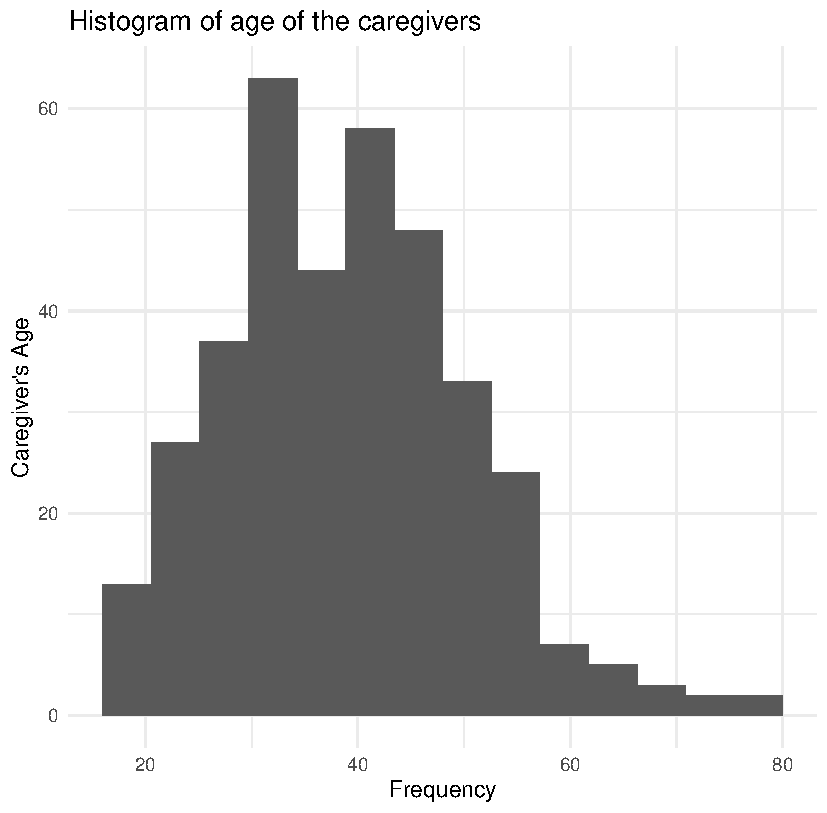
\includegraphics[scale=0.4]{Rplot01.pdf}
		\end{column}
		
		\begin{column}{0.4\textwidth}
			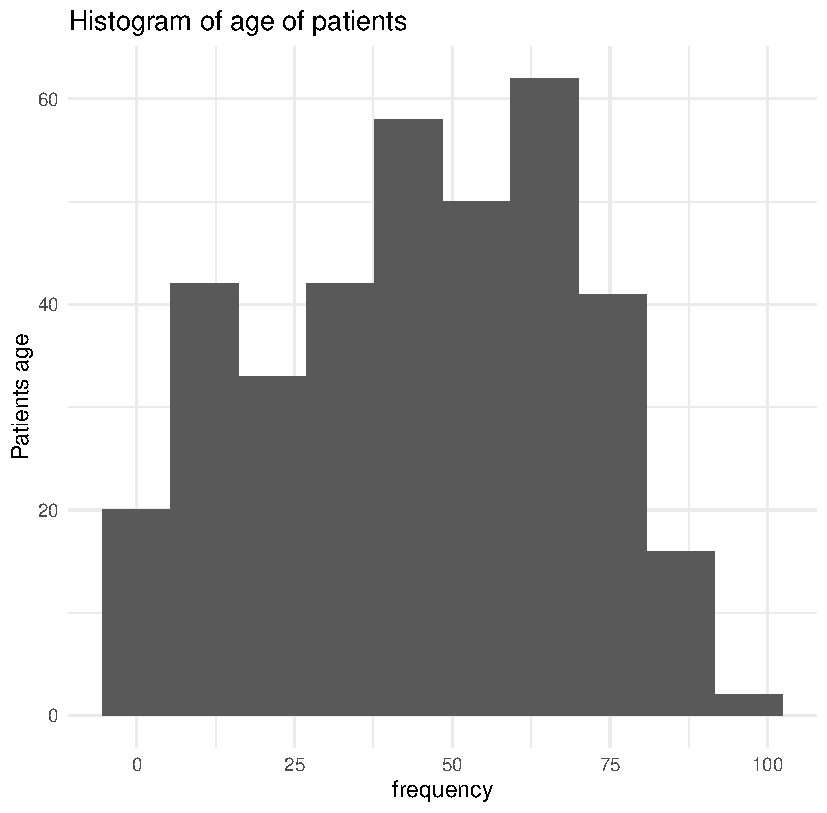
\includegraphics[scale=0.4]{Rplot02.pdf}
		\end{column}
		
	\end{columns}
\end{frame}
\begin{frame}
\begin{itemize}
\item Before we conduct multiple linear regression,we check if the data meets the assumptions of a multiple linear regression.
\vspace{4mm}
\item One of the assumptions is the multivariate normality.

\vspace{4mm}
\item To do this, we use the chi-square plot to plot the squared Mahalanobis distance to assess this assumption.
\end{itemize}
\end{frame}
\begin{frame}
	\begin{columns}[c]
	\begin{column}{0.6\textwidth}
		
		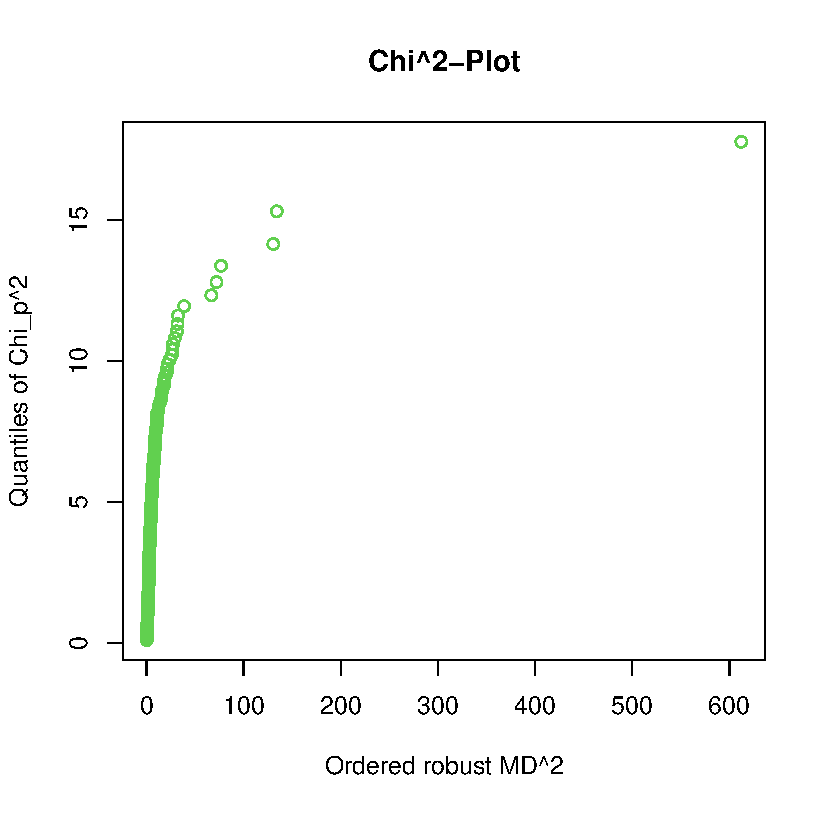
\includegraphics[scale=0.5]{Rplot03.pdf}
	\end{column}
	
	\begin{column}{0.4\textwidth}
\begin{block}{.}
 From the plot, the data is not multivariate normal. Hence we normalize the data by taking natural log of the independent random variables to minimize on the effects of the outliers in the dataset.
 \end{block}
\end{column}
	
\end{columns}
\end{frame}

\begin{frame}
\noindent \underline{\textbf{Multivariate normality check of the transformed data}}
\begin{adjustbox}{max width=\textwidth}
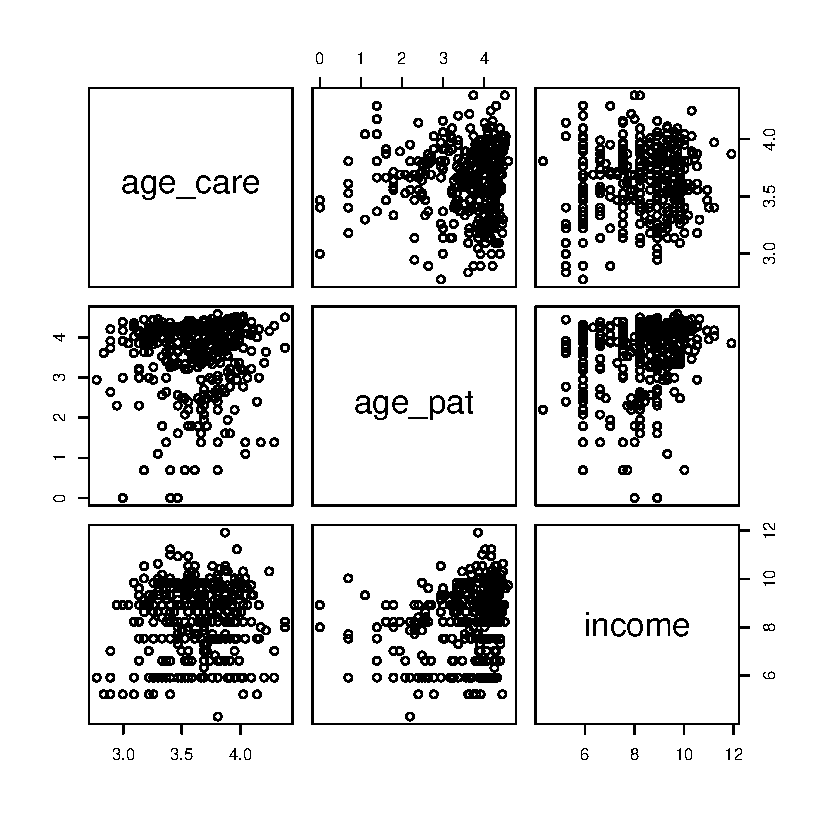
\includegraphics[scale=0.6]{Rplot04.pdf}
\end{adjustbox}
\end{frame}

\begin{frame}	

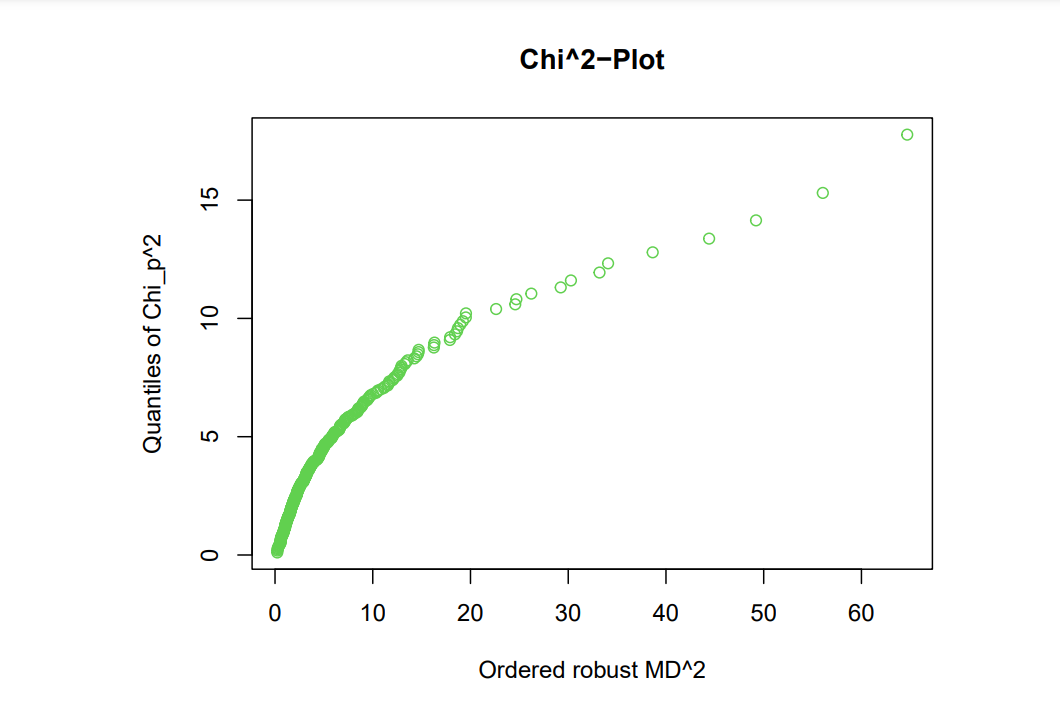
\includegraphics[scale=0.5]{Rplot05.png}
\begin{block}{.}
From the pairs plot, the data form ellipsoid clusters implying the data is multivariate normal as it is confirmed also by the squared Mahalanobis' distance plot.\\~\\
\end{block}
\end{frame}

\begin{knitrout}
	\begin{adjustbox}{max width=\textwidth}

	\definecolor{shadecolor}{rgb}{0.969, 0.969, 0.969}\color{fgcolor}\begin{kframe}
		\begin{alltt}
			\hlstd{data1}\hlkwb{<-}\hlkwd{as.data.frame}\hlstd{(data_trans)}
			\hlstd{Model}\hlkwb{<-}\hlkwd{lm}\hlstd{(PHQ}\hlopt{~}\hlstd{age_care}\hlopt{+}\hlstd{age_pat}\hlopt{+}\hlstd{income,} \hlkwc{data} \hlstd{= data1)}
			\hlkwd{summary}\hlstd{(Model)}
		\end{alltt}
		\begin{verbatim}

			## Coefficients:
			##             Estimate Std. Error t value Pr(>|t|)    
			## (Intercept)  11.3014     2.3971   4.715 3.47e-06 ***
			## age_care     -0.2735     0.5941  -0.460 0.645547    
			## age_pat      -0.7151     0.2079  -3.440 0.000649 ***
			## income       -0.4352     0.1286  -3.385 0.000791 ***
			## ---
			## Residual standard error: 3.409 on 361 degrees of freedom
			## Multiple R-squared:  0.7711,	Adjusted R-squared:  0.6944 
			## F-statistic: 10.05 on 3 and 361 DF,  p-value: 2.23e-06
		\end{verbatim}
		\begin{alltt}
			\hlcom{#anova(Model)}
		\end{alltt}
	\end{kframe}
		\end{adjustbox}
\end{knitrout}

\begin{frame}{Multiple linear Regression model}
	
\begin{block}{.}
	\begin{itemize}
\item  The model adopted  $\tilde{Y}=\beta_{0}+\beta_{i}log X$.
\vspace{2mm}
\item On the implied model, 1\% change in X leads to approximately $\beta_{i}$/100 unit change in $Y$
\vspace{2mm}
\item  The estimated model is:
$$\tilde{y}=11.3014-0.2735x_{1}-0.7151x_{2}-0.4352x_{3}$$
	\end{itemize}
\end{block}

\end{frame}

\subsection{Data interpretation and Discussions}
\begin{frame}{Model Evaluation}
	\begin{block}{.}
 At 95\% significance, the intercept and age of the patient and income levels of the care givers are significant in determining the PHQ levels of the care giver. As noted, the age of the care giver is not significant in determining the PHQ levels of the care giver.\\
	\end{block}
\end{frame}

\begin{frame}
\begin{block}{Age of the caregiver}
With age of the patient and house hold income held constant, 1\% change in age of the care giver leads to approximately (-0.2735)/100 unit change in the PHQ levels.
\end{block}


\vspace{0.2cm}
\begin{block}{Age of patient}
With Age of the caregiver and the household income held constant, 1\% change in age of the age of the patient leads to approximately (-0.7151 )/100 unit change in the PHQ levels.
\end{block}
\vspace{0.2cm}
\begin{block}{Household Income}
Holding the age of the patient and the age of the caregiver constant, 1\% change in income  of the care giver leads to approximately (-0.4352)/100 unit change in in the PHQ levels.
\end{block}

\end{frame}

\begin{frame}{Diagnostics}
\begin{block}{i. Linearity}
	We test that assumption that the model is linaer with respect to $\beta_{i} 's$
\end{block}
	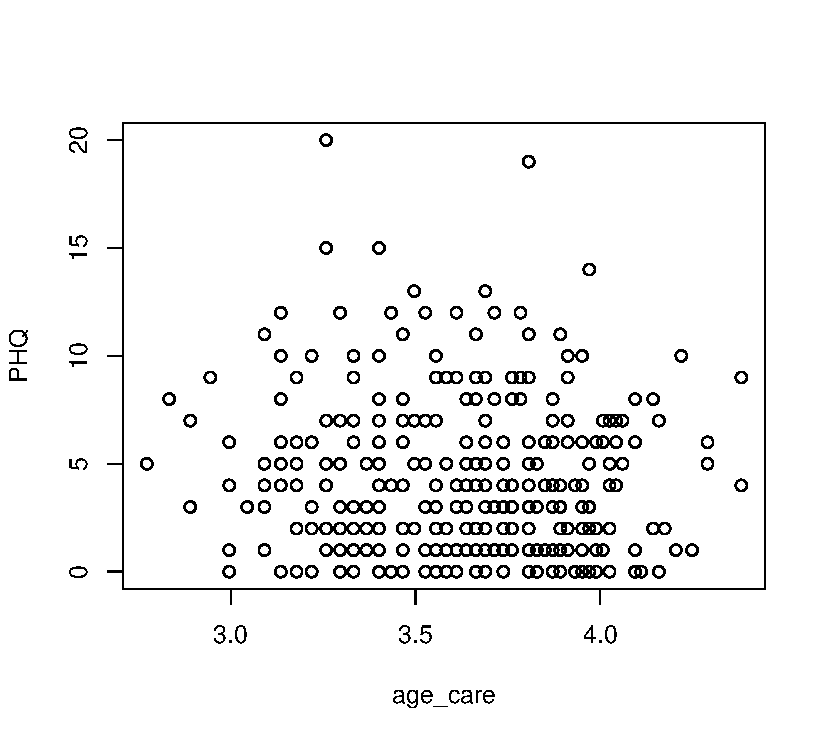
\includegraphics[scale=0.5]{Rplot06.pdf} 
	
\end{frame}
\begin{frame}
	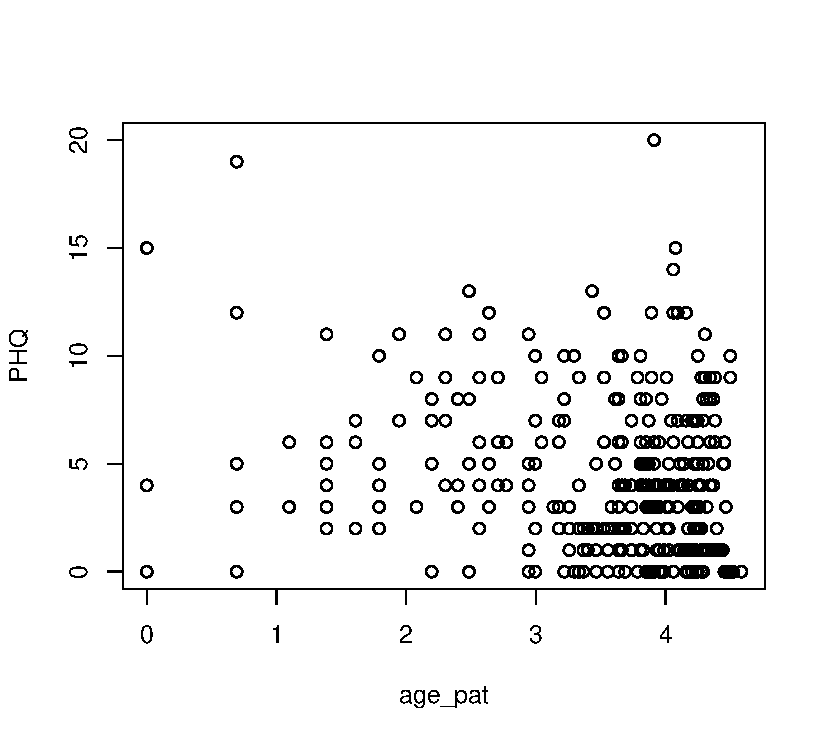
\includegraphics[scale=0.6]{Rplot07.pdf} 

	\begin{block}{.}
There is a linear relationship between the dependent variables and independent variables.
	\end{block}
\end{frame}
\begin{frame}
	
\noindent \textbf{Normality of the residuals}
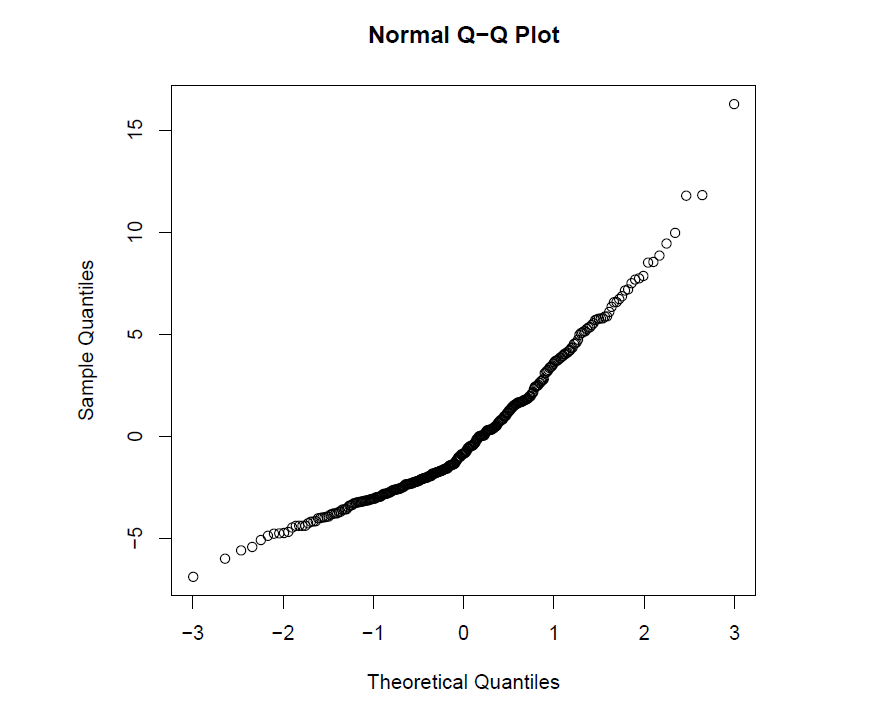
\includegraphics[scale=0.6]{Rplot09.png} \\
\begin{block}{.}
The qqnorm plot shows the residuals are normally distributed.
\end{block}
\end{frame}

\begin{frame}
\noindent \textbf{ii.Homoscedasticity}
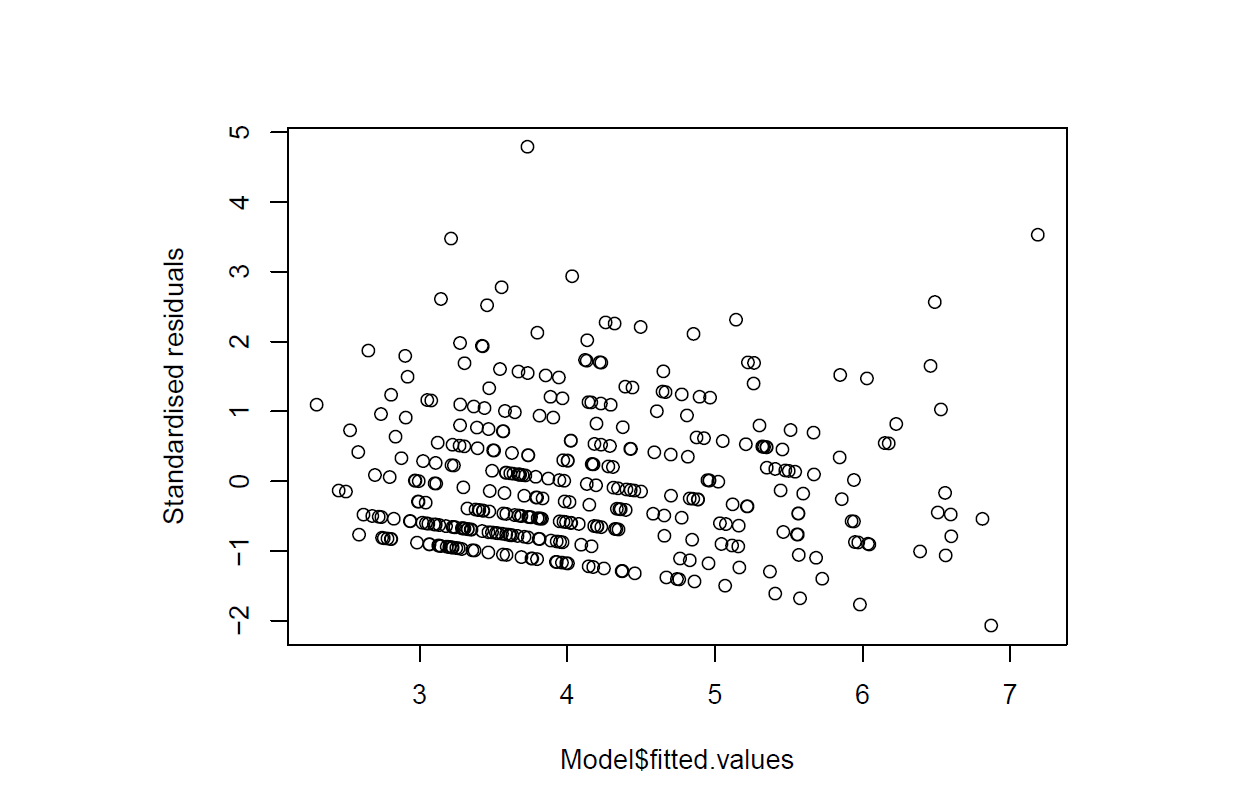
\includegraphics[scale=0.5]{Rplot10.png} 
\begin{block}{.}
The variance of the the errors is constant across all the levels as evidenced by the plot above since the residuals have  a constant mean of zero.
\end{block}
\end{frame}
\begin{block}{Multi colinearity diagnostics}
\noindent Test of no multi-colinearity
\end{block}
\begin{block}{.}
\begin{knitrout}
	\definecolor{shadecolor}{rgb}{0.969, 0.969, 0.969}\color{fgcolor}\begin{kframe}
		\begin{alltt}
			\hlkwd{library}\hlstd{(car)}
			\hlkwd{vif}\hlstd{(Model)}
		\end{alltt}
		\begin{verbatim}
			## age_care  age_pat   income 
			## 1.003792 1.048467 1.052330
		\end{verbatim}
	\end{kframe}
\end{knitrout}
\noindent Each independent variable has a Variance inflation factor of 1 indicating no correlation between the independent variable and other variables in the model.\\~\\
\end{block}
\section{Conclusion and Recommendation}
\begin{frame}{Conclusion}
	\begin{itemize}
		\item The age of patient and level of income are significant in determining the level of depression of cancer caregivers in that the level of depression decreases with increase in age of a patient as well as increase of level of income of a caregiver. The age of the cancer caregiver is insignificant.
		\item Income has a stronger correlation with the  level of depression than age. However, there may be other qualitative factors not considered in the analysis that contribute to the remaining percentage of fitness such as support groups and level of education
	\end{itemize}
\end{frame}
\begin{frame}{Recommendations}
	\begin{itemize}
		\item We recommend for more variables to be used in future research to get a more accurate model i.e. qualitative variable support groups,level of education et al.
		\item For easier availability of cancer caregivers data in Kenya, Kenya National Bureau  of Statistics to conduct such research and make the data available online for future research.
		\item Given the role being played by cancer caregivers, the government through state departments should develop intervetions and tailored support to cancer caregivers for better quality of life of the patients.
	\end{itemize}
\end{frame}
\begin{frame}{References}
	\begin{enumerate}
\item Jain G., Roy A., Harikrishnan V., Yu S., Dabbous O. and Lawrence, C. (2013), Patient-Reported Depression Severity Measured by the PHQ-9 and Impact on Work Productivity, \emph{Journal of Occupational and Environmental Medicine}, 55(3), 252-258.
\item Kaggwa M. M., Najjuka, S. M., Nuwamanya S., Nabulo, H., and Nkola R. (2021). Depression among cancer caregivers in a rural setting.xlsx. Retrieved from
\href{https://figshare.com/articles/dataset/Depressionamongcancercaregiversinaruralsettingxlsx/doi: 10.6084/m9.figshare.14524800.v1}{figshare}

\item Laing S. S., and Jones S. M. (2016), Anxiety and Depression Mediate the Relationship between Perceived Workplace Health Support and Presenteeism, \emph{Journal of Occupational and Environmental Medicine}, 58(11), 1144-1149.

\item Leung D. Y., Mak Y. W., Leung S. F., Chiang V. C. and Loke A. Y. (2020), Measurement Invariances of the PHQ‐9 Across Gender and Age Groups in Chinese Adolescents,\emph{ Asia‐Pacific Psychiatry}, 12(3), e12381.
\seti
\end{enumerate}
\end{frame}
\begin{frame}
	\begin{enumerate}
		\conti
\item Levis B., Benedetti A. and Thombs B. D. (2019), Accuracy of Patient Health Questionnaire-9 (PHQ-9) For Screening to Detect Major Depression: Individual Participant Data Meta-Analysis,\emph{BMJ}, 365.

\item Levis B., Sun Y., He C., Wu Y., Krishnan A., Bhandari P. M. and Thombs B. D. (2020), Accuracy of the PHQ-2 Alone and in Combination with the PHQ-9 for Screening to Detect Major Depression: Systematic Review and Meta-Analysis,\emph{ JAMA}, 323(22), 2290-2300.

\item Lister K., Seale J. and Douce C. (2023), Mental Health in Distance Learning: A Taxonomy of Barriers and Enablers to Student Mental Wellbeing, \emph{Open Learning: The Journal of Open, Distance and e-Learning}, 38(2), 102-116.

\item Magtibay D. L., Chesak S. S., Coughlin K. and Sood, A. (2017), Decreasing Stress and Burnout in Nurses, \emph{The Journal of Nursing Administration}, 47(7/8), 391-395.

\seti
	\end{enumerate}
\end{frame}
\begin{frame}
	\begin{enumerate}
	\conti
\item Martin A., Sanderson K. and Cocker F. (2009), Meta-Analysis of the Effects of Health Promotion Intervention in the Workplace on Depression and Anxiety Symptoms,\emph{Scandinavian Journal of Work, Environment and Health}, 7-18.
\item  Montgomery C. D, Peck A. E and Vining G.G.(2012), Introduction to linear regression analysis, John Wiley \& Sons Inc.
\item Serpa J. G., Taylor S. L. and Tillisch K. (2014), Mindfulness-Based Stress Reduction (MBSR) Reduces Anxiety, Depression, and Suicidal Ideation in Veterans, \emph{Medical Care}, 52(12), S19-S24.
	\end{enumerate}
\end{frame}
\begin{frame}
	\begin{center}
		{\fontsize{40}{50}\selectfont Thank You!}
	\end{center}
\end{frame}
\end{document}